\section{An \pdfEinfty-structure on cubical chains} \label{s:action}

In this section we construct a natural $\M$-bialgebra structure on the chains of representable cubical sets.
These are determined by three natural linear maps satisfying the relations defining $\mathcal M$.
A Yoneda extension then provides the chains of any cubical set with a natural $\UM$-coalgebra structure.
We begin by recalling the basics of cubical topology.

\subsection{Cubical sets}

The objects of the \textit{cube category} $\cube$ are the sets $2^n = \{0, 1\}^n$ with $2^0 = \{0\}$ for $n \in \N$, and its morphisms are generated by the \textit{coface} and \textit{codegeneracy} maps
\begin{align*}
\delta_i^\varepsilon & = \mathrm{id}_{2^{i-1}} \times \delta^\varepsilon \times \mathrm{id}_{2^{n-1-i}} \colon 2^{n-1} \to 2^n, \\
\sigma_i & = \mathrm{id}_{2^{i-1}} \times \, \sigma \times \mathrm{id}_{2^{n-i}} \quad \colon 2^{n} \to 2^{n-1},
\end{align*}
where $\varepsilon \in \{0,1\}$ and the functors
\[
\begin{tikzcd} [column sep=16pt]
2^0 \arrow[r, bend left, "\delta^0"] \arrow[r, bend right, "\delta^1"'] & 2^1 \arrow[r, "\sigma"] & 2^0
\end{tikzcd}
\]
are defined by
\[
\delta^0(0) = 0, \qquad \delta^1(0) = 1, \qquad \sigma(0) = \sigma(1) = 0.
\]
More globally, the category $\cube$ is the free strict monoidal category with an assigned internal bipointed object.
We refer to \cite{grandis2003cubical} for a more leisurely exposition and variants of this definition.

We denote by $\mathrm{Dgn}(2^m, 2^n)$ the subset of morphism in $\cube(2^m, 2^n)$ of the form $\sigma_i \circ \tau$ with $\tau \in \cube(2^m, 2^{n+1})$.

The category of \textit{cubical sets} $\Fun(\cube^\op, \Set)$ is denoted by $\cSet$ and the representable cubical set $\yoneda(2^n)$ by $\cube^n$.
For any cubical set $X$ we write, as usual, $X_n$ instead of $X(2^n)$.

\subsection{Cubical topology}

Consider the topological $n$-cube
\[
\gcube^{n} = \big\{ (x_1, \dots, x_n) \mid x_i \in [0,1] \big\}.
\]
The assignment $2^n \to \gcube^n$ defines a functor $\cube \to \Top$ with
\begin{align*}
\delta^\varepsilon_i(x_1, \dots, x_n) &= (x_1, \dots, x_i, \varepsilon, x_{i+1}, \dots x_n), \\
\sigma_i(x_1,\dots,x_n) &= (x_1, \dots, \widehat{x}_i, \dots, x_n).
\end{align*}
Its Yoneda extension is known as \textit{geometric realization}.
It has a right adjoint $\cSing \colon \Top \to \cSet$ referred to as the \textit{cubical singular complex} satisfying
\[
\cSing(\fZ)_n = \Top(\gcube^n, \fZ)
\]
for any topological space $\fZ$.

\subsection{Cubical chains}

The functor of (\textit{normalized}) \textit{chains} $\chains \colon \cSet \to \Ch$ is the Yoneda extension of the functor $\cube \to \Ch$ defined next.
It assigns to an object $2^n$ the chain complex having in degree $m$ the module
\[
\frac{\k\{\cube(2^m, 2^n)\}}{\k\{\mathrm{Dgn}(2^m, 2^n)\}}
\]
and differential induced by
\[
\bd (\id_{2^n}) = \sum_{i=1}^{n} \ (-1)^i \
\big(\delta_i^1 - \delta_i^0 \big).
\]
To a morphism $\tau \colon 2^n \to 2^{n'}$ it assigns the chain map
\[
\begin{tikzcd}[row sep=-3pt, column sep=normal,
/tikz/column 1/.append style={anchor=base east},
/tikz/column 2/.append style={anchor=base west}]
\chains(\cube^n)_m \arrow[r] & \chains(\cube^{n'})_m \\
\big( 2^m \to 2^n \big) \arrow[r, mapsto] & \big( 2^m \to 2^n \stackrel{\tau}{\to} 2^{n'} \big).
\end{tikzcd}
\]
The chain complex $\chains(\cube^n)$ is isomorphic to both: $\chains(\cube^1)^{\ot n}$ and the cellular chains on the topological $n$-cube with its standard CW structure $\gchains(\gcube^n)$.
We use the isomorphism $\chains(\cube^n) \cong \gchains(\gcube^1)^{\ot n}$ when denoting the elements in the basis of $\chains(\cube^n)$ by $x_1 \ot \dotsb \ot x_n$ with $x_i \in \{[0], [0,1], [1]\}$.

For a topological space $\fZ$, the chain complex $\chains(\cSing \fZ)$ is referred to as the \textit{cubical singular chains} of $\fZ$.

\subsection{Serre coalgebra} \label{ss:serre coalgebra}

We now recall the \textit{Serre coalgebra structure}, a natural (counital and coassociative) coalgebra structure on cubical chains.

By a Yoneda extension, to define this structure it suffices to describe it on the chains of representable cubical sets $\chains(\cube^n)$.
For $\chains(\cube^1)$ we have
\begin{align*}
	\epsilon \big([0]\big) &= 1,
	& \Delta \big([0]\big) &= [0] \ot [0], \\
	\epsilon \big([1]\big) &= 1,
	& \Delta \big([1]\big) &= [1] \ot [1], \\
	\epsilon \big([0,1]\big) &= 0,
	& \Delta \big([0,1]\big) &= [0] \ot [0,1] + [0,1] \ot [1].
\end{align*}
The Serre coalgebra structure on a general $\chains(\cube^n)$ is define using the isomorphism $\chains(\cube^n) \cong \chains(\cube^1)^{\ot n}$ and the monoidal structure on the category of coalgebras.
Explicitly, the structure maps are given by the compositions
\[
\epsilon \colon \chains(\cube^1)^{\ot n} \xra{\epsilon^{\ot n}} \k^{\ot n} \to \k
\]
and
\[
\Delta \colon \chains(\cube^1)^{\ot n} \xra{\Delta^{\!\ot n}} \left( \chains(\cube^1)^{\ot 2} \right)^{\ot n} \xra{\sigma_{2n}^{-1}} \left( \chains(\cube^1)^{\ot n} \right)^{\ot 2},
\]
where $\sigma_{2n}$ in $\sym_{2n}$ is the $(n,n)$-shuffle mapping the first and second ``decks'' to odd and even values respectively.
An explicit description of $\sigma_{2n}$ is presented in \cref{e:shuffle perm}.

\begin{remark*}
	Similarly to how the Alexander--Whitney coalgebra can be interpreted geometrically as the sum of all complementary pairs of front and back faces of a simplex, this coproduct is, up to signs, also given by the sum of complementary pairs of front and back faces of a cube.
\end{remark*}

For later reference we record a useful description of the value of $\Delta$ on the top dimensional basis element of $\chains(\cube^n)$.

\begin{lemma} \label{l:coproduct description}
	For any $n \in \N$,
	\[
	\Delta \big( [0,1]^{\ot n} \big) =
	\sum_{\lambda \in \Lambda} (-1)^{\ind \lambda} \
	\Big(x_1^{(\lambda)} \ot \cdots \ot x_n^{(\lambda)}\Big) \ot
	\Big(y_1^{(\lambda)} \ot \cdots \ot y_n^{(\lambda)}\Big),
	\]
	where each $\lambda$ in $\Lambda$ is a map $\lambda \colon \{1,\dots,n\} \to \set{0, 1}$ with $\lambda(i)$ interpreted as
	\begin{align*}
		0:\ \, x_i^{(\lambda)} &= [0,1], &	1: \ \, x_i^{(\lambda)} &= [0], \\
		y_i^{(\lambda)} &= [1],  & y_i^{(\lambda)} &= [0,1],
	\end{align*}
	and $\ind \lambda$ is the cardinality of $\set{i<j \mid \lambda(i) > \lambda(j)}$.
\end{lemma}

\subsection{Degree 1 product}

Let $n \in \N$.
For $x = x_1 \ot \dotsb \ot x_n$ a basis element of $\chains(\cube^n)$ and $\ell \in \set{1,\dots,n}$ we write
\begin{align*}
	x_{<\ell} & = x_1 \ot \dotsb \ot x_{\ell-1}, \\
	x_{>\ell} & = x_{\ell+1} \ot \dotsb \ot x_n,
\end{align*}
with the convention
\[
x_{<1} = x_{>n} = 1 \in \Z.
\]
We define the \textit{product} $\ast \colon \chains(\square^n)^{\ot 2} \to \chains(\square^n)$ by
\begin{multline*}
(x_1 \ot \dotsb \ot x_n) \ast (y_1 \ot \dotsb \ot y_n)
=
(-1)^{|x|} \sum_{i=1}^n x_{<i}\, \epsilon(y_{<i}) \ot x_i \ast y_i \ot \epsilon(x_{>i}) \, y_{>i},
\end{multline*}
where the only non-zero values of $x_i \ast y_i$ are
\[
[0] \ast [1] = [0, 1], \qquad [1] \ast [0] = -[0, 1].
\]

\begin{example*}
	Since in $\chains(\cube^3)$ we have that
	\[
	\bd \big([0]\ot[0]\ot[0]\big) = \bd \big([1]\ot[1]\ot[1]\big) = 0
	\]
	and
	\begin{multline*}
		\bd\big([0]\ot[0]\ot[0] \ast [1]\ot[1]\ot[1]\big) \\ =
		\bd\big([0,1]\ot[1]\ot[1] + [0]\ot[0,1]\ot[1] + [0]\ot[0]\ot[0,1] \big) \\ =
		[1]\ot[1]\ot[1] - [0]\ot[0]\ot[0],
	\end{multline*}
	we conclude that in general $\ast$ is not a cycle in the appropriate Hom complex, so it does not descend to homology.
	This product should be understood as an algebraic version of a consistent choice of path between points in a cube.
	In our case, as illustrated in \cref{f:product}, the chosen path is given by the union of segments parallel to edges of the cube.
\end{example*}

\begin{figure}[h!]
	\centering
	\documentclass{standalone}
\usepackage{tikz}
\usepackage{amsmath}

\begin{document}
	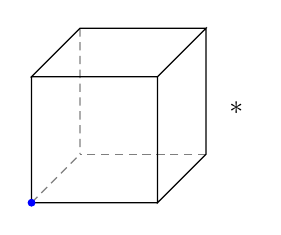
\begin{tikzpicture}[every edge quotes/.append style={auto, text=black}, scale=.4]
		\pgfmathsetmacro{\cubex}{4}
		\pgfmathsetmacro{\cubey}{4}
		\pgfmathsetmacro{\cubez}{4}
		\draw [draw=black, every edge/.append style={draw=black, densely dashed, opacity=.5}, fill=white]
		(0,0,0) coordinate (o) -- ++(-\cubex,0,0) coordinate (a) -- ++(0,-\cubey,0) coordinate (b) edge coordinate [pos=1] (g) ++(0,0,-\cubez) -- ++(\cubex,0,0) coordinate (c) -- cycle
		(o) -- ++(0,0,-\cubez) coordinate (d) -- ++(0,-\cubey,0) coordinate (e) edge (g) -- (c) -- cycle
		(o) -- (a) -- ++(0,0,-\cubez) coordinate (f) edge (g) -- (d) -- cycle;
		\path [every edge/.append style={draw=black, |-|}];

		\draw [blue,fill] (b) circle [radius=3pt];
		\draw[] node at (2.5,-1){$\ast$};
	\end{tikzpicture}
	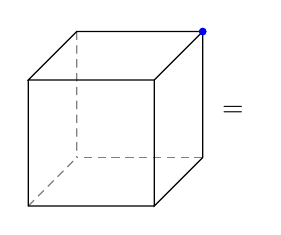
\begin{tikzpicture}[every edge quotes/.append style={auto, text=black}, scale=.4]
		\pgfmathsetmacro{\cubex}{4}
		\pgfmathsetmacro{\cubey}{4}
		\pgfmathsetmacro{\cubez}{4}
		\draw [draw=black, every edge/.append style={draw=black, densely dashed, opacity=.5}, fill=white]
		(0,0,0) coordinate (o) -- ++(-\cubex,0,0) coordinate (a) -- ++(0,-\cubey,0) coordinate (b) edge coordinate [pos=1] (g) ++(0,0,-\cubez) -- ++(\cubex,0,0) coordinate (c) -- cycle
		(o) -- ++(0,0,-\cubez) coordinate (d) -- ++(0,-\cubey,0) coordinate (e) edge (g) -- (c) -- cycle
		(o) -- (a) -- ++(0,0,-\cubez) coordinate (f) edge (g) -- (d) -- cycle;
		\path [every edge/.append style={draw=black, |-|}];

		\draw [blue, fill] (d) circle [radius=3pt];
		\draw[] node at (2.5,-1){$=$};
	\end{tikzpicture}
	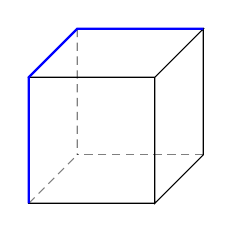
\begin{tikzpicture}[every edge quotes/.append style={auto, text=black}, scale=.4]
		\pgfmathsetmacro{\cubex}{4}
		\pgfmathsetmacro{\cubey}{4}
		\pgfmathsetmacro{\cubez}{4}
		\draw [draw=black, every edge/.append style={draw=black, densely dashed, opacity=.5}, fill=white]
		(0,0,0) coordinate (o) -- ++(-\cubex,0,0) coordinate (a) -- ++(0,-\cubey,0) coordinate (b) edge coordinate [pos=1] (g) ++(0,0,-\cubez) -- ++(\cubex,0,0) coordinate (c) -- cycle
		(o) -- ++(0,0,-\cubez) coordinate (d) -- ++(0,-\cubey,0) coordinate (e) edge (g) -- (c) -- cycle
		(o) -- (a) -- ++(0,0,-\cubez) coordinate (f) edge (g) -- (d) -- cycle;
		\path [every edge/.append style={draw=black, |-|}];

		\draw[blue, thick] (b)--(a)--(f)--(d);
	\end{tikzpicture}
\end{document}
	\caption{Geometric representation of $\big([0]\ot[0]\ot[0] \ast [1]\ot[1]\ot[1]\big)$ where we are using the width-depth-height order.}
	\label{f:product}
\end{figure}

\subsection{$\M$-bialgebra on representable cubical sets}

\begin{lemma} \label{l:cubical chain bialgebra}
	The assignment
	\[
	\counit \mapsto \epsilon, \quad \coproduct \mapsto \Delta, \quad \product \mapsto \ast,
	\]
	induces a natural $\mathcal M$-bialgebra structure on $\chains(\square^n)$ for every $n \in \N$.
\end{lemma}

\begin{proof}
	We need to show that this assignment is compatible with the relations
	\[
	\productcounit = 0, \qquad
	\leftcounitality = 0, \qquad
	\rightcounitality = 0,
	\]
	and
	\[
	\bd\ \counit = 0, \qquad
	\bd\ \coproduct = 0, \qquad
	\bd\ \product = \ \boundary\,.
	\]
	For the rest of this proof let us consider two basis elements of $\chains(\square^n)$
	\begin{align*}
		x = x_1 \ot \dotsb \ot x_n
		\qquad \text{ and } \qquad
		y = y_1 \ot \dotsb \ot y_n.
	\end{align*}
	Since the degree of $\ast$ is $1$ and $\epsilon([0,1]) = 0$, we can verify the first relation easily:
	\begin{align*}
		\varepsilon(x \ast y) & =
		\sum (-1)^{|x|} \epsilon(y_{<i}) \epsilon(x_{<i}) \ot \epsilon(x_i \ast y_i) \ot \epsilon(x_{>i}) \epsilon(y_{>i}) = 0.
	\end{align*}
	For the second relation we want to show that $(\epsilon \ot \id) \circ \Delta = \id$.
	Since
	\begin{gather*}
		(\epsilon \ot \id) \circ \Delta([0]) = \epsilon([0]) \ot [0] = [0], \\
		(\epsilon \ot \id) \circ \Delta([1]) = \epsilon([1]) \ot [1] = [1], \\
		(\epsilon \ot \id) \circ \Delta([0, 1]) = \epsilon([0]) \ot [0, 1] + \epsilon([0, 1]) \ot [1] = [0,1],
	\end{gather*}
	we have
	\begin{multline*}
		(\epsilon \ot \id) \circ \Delta (x_1 \ot \dotsb \ot x_n) = \\
		\sum \pm \left( \epsilon \big(x_1^{(1)}\big) \ot \dotsb \ot \epsilon\big(x_n^{(1)}\big) \right) \ot
		\left( x_1^{(2)} \ot \dotsb \ot x_n^{(2)} \right) \\ =
		x_1 \ot \dotsb \ot x_n,
	\end{multline*}
	where the sign is obtained by noticing that the only non-zero term occurs when each factor $x_i^{(0)}$ is of degree $0$.
	The third relation is verified analogously.
	The fourth and fifth are precisely the well known facts that $\epsilon$ and $\Delta$ are chain maps.
	To verify the sixth and final relation we need to show that
	\[
	\bd (x \ast y)\ +\ \bd x \ast y\ +\ (-1)^{|x|}x \ast \bd y\ =\ \epsilon(x) y \ -\ \epsilon(y) x.
	\]
	We have
	\[
	x \ast y = \sum (-1)^{|x|} x_{<i} \, \epsilon(y_{<i}) \ot x_i \ast y_i \ot \epsilon(x_{>i})\, y_{>i}
	\]
	and
	\begin{align*}
		\bd(x \ast y) & =
		\sum (-1)^{|x|} \, \bd x_{<i}\, \epsilon(y_{<i}) \ot x_i \ast y_i \ot \epsilon(x_{>i})\, y_{>i} \\ & +
		\sum (-1)^{|x|+|x_{<i}|} \, x_{<i}\, \epsilon(y_{<i}) \ot \bd (x_i \ast y_i) \ot \epsilon(x_{>i}) \, y_{>i} \\ & -
		\sum (-1)^{|x|+|x_{<i}|} \, x_{<i}\, \epsilon(y_{<i}) \ot x_i \ast y_i \ot \epsilon(x_{>i})\, \bd y_{>i}.
	\end{align*}
	Since $|x| = |x_{<i}| + |x_i| + |x_{>i}|$ and $\epsilon(x_{>i}) \neq 0 \Leftrightarrow |x_{>i}| = 0$ as well as $\bd(x_i \ast y_i) \neq 0 \Rightarrow |x_i| = 0$
%	\[
%	|x| = |x_{<i}| + |x_i| + |x_{>i}|, \quad \epsilon(x_{>i}) \neq 0 \Leftrightarrow |x_{>i}| = 0, \quad \bd(x_i \ast y_i) \neq 0 \Rightarrow |x_i| = 0,
%	\]
	we have
	\begin{equation} \label{e:boundary of product 1}
		\begin{split}
			\bd(x \ast y) & =
			\sum (-1)^{|x|} \, \bd x_{<i}\, \epsilon(y_{<i}) \ot x_i \ast y_i \ot \epsilon(x_{>i})\, y_{>i} \\ & +
			\sum x_{<i} \, \epsilon(y_{<i}) \ot \bd (x_i \ast y_i) \ot \epsilon(x_{>i})\, y_{>i} \\ & -
			\sum x_{<i} \, \epsilon(y_{<i}) \ot x_i \ast y_i \ot \epsilon(x_{>i})\, \bd y_{>i}.
		\end{split}
	\end{equation}
	We also have
	\begin{align*}
		\bd x \ast y & =
		\sum (-1)^{|x|-1} \, \bd x_{<i}\, \epsilon(y_{<i}) \ot x_i \ast y_i \ot \epsilon(x_{>i}) \, y_{>i} \\ & +
		\sum (-1)^{|x|-1+|x_{<i}|} \, x_{<i}\, \epsilon(y_{<i}) \ot \bd x_i \ast y_i \ot \epsilon(x_{>i}) \, y_{>i} \\ & +
		\sum (-1)^{|x|-1+|x_{<i}|} \, x_{<i}\, \epsilon(y_{<i}) \ot x_i \ast y_i \ot \epsilon(\bd x_{>i}) \, y_{>i}.
	\end{align*}
	Since
	\[
	\epsilon(\bd x_{>i}) = 0, \quad \bd x_i \neq 0 \Leftrightarrow |x_i| = 1,
	\]
	we have
	\begin{equation} \label{e:boundary of product 2}
		\begin{split}
			\bd x \ast y & =
			\sum (-1)^{|x|-1} \, \bd x_{<i}\, \epsilon(y_{<i}) \ot x_i \ast y_i \ot \epsilon(x_{>i})\, y_{>i} \\ & +
			\sum x_{<i}\, \epsilon(y_{<i}) \ot \bd x_i \ast y_i \ot \epsilon(x_{>i})\, y_{>i}.
		\end{split}
	\end{equation}
	We also have
	\begin{align*}
		(-1)^{|x|} \, x \ast \bd y & =
		\sum x_{<i} \, \epsilon(\bd y_{<i}) \ot x_i \ast y_i \ot \epsilon(x_{>i})\, y_{>i} \\ & +
		\sum (-1)^{|y_{<i}|} \, x_{<i}\, \epsilon(y_{<i}) \ot x_i \ast \bd y_i \ot \epsilon(x_{>i}) \, y_{>i} \\ & +
		\sum (-1)^{|y_{<i}| + |y_i|} \, x_{<i}\, \epsilon(y_{<i}) \ot x_i \ast y_i \ot \epsilon(x_{>i}) \, \bd y_{>i},
	\end{align*}
	which is equivalent to
	\begin{equation} \label{e:boundary of product 3}
		\begin{split}
			(-1)^{|x|} \, x \ast \bd y & =
			\sum x_{<i} \, \epsilon(y_{<i}) \ot x_i \ast \bd y_i \ot \epsilon(x_{>i})\, y_{>i} \\ & +
			\sum x_{<i}\, \epsilon(y_{<i}) \ot x_i \ast y_i \ot \epsilon(x_{>i})\, \bd y_{>i}.
		\end{split}
	\end{equation}
	Putting identities \eqref{e:boundary of product 1}, \eqref{e:boundary of product 2} and \eqref{e:boundary of product 3} together, we get
	\begin{multline*}
		\bd (x \ot y) \ +\ \bd x \ast y\ +\, (-1)^{|x|}x \ast \bd y \\
		= \sum \epsilon(y_{<i})\, x_{<i} \ot \big(\bd(x_i \ast y_i) + \bd x_i \ast y_i + x_i \ast \bd y_i\big) \ot \epsilon(x_{>i})\, y_{>i}.
	\end{multline*}
	Since
	\begin{align*}
		\bd(x_i \ast y_i)\ +\ \bd x_i \ast y_i\ +\ x_i \ast \bd y_i =
		\epsilon(x_i)y_i\ -\ \epsilon(y_i)x_i,
	\end{align*}
	we have
	\begin{multline*}
		\bd (x \ast y) \ +\ \bd x \ast y\ +\ (-1)^{|x|}x \ast \bd y = \\
		\sum \epsilon(y_{<i}) \, x_{<i} \ot \epsilon(x_{\geq i}) y_{\geq i}\ -\
		\epsilon(y_{\leq i}) \, x_{\leq i} \ot \epsilon(x_{>i}) y_{>i} \\ =
		\epsilon(x)y - \epsilon(y)x,
	\end{multline*}
	as desired, where the last equality follows from a telescopic sum argument.
\end{proof}

\subsection{$\texorpdfstring{E_\infty}{E-infty}$-coalgebra on cubical chains}

\cref{l:cubical chain bialgebra} defines a functor from the cube category to that of $\M$-bialgebras.
This category is not cocomplete so we do not expect to have an $\M$-bialgebra structure on arbitrary cubical sets.
For example, consider the chains on the cubical set $X$ whose only non-degenerate simplices are $v, w \in X_0$.
By degree reasons $v \ast w = 0$ for any degree 1 product $\ast$ in $\chains(X)$.
The third relation in $\M$ would then imply the contradiction $0 = w-v$.
Since categories of coalgebras over operads are cocomplete we have the following.

\begin{theorem} \label{t:lift to e infinity coalgebras}
	The Yoneda extension of the composition of the functor $\cube \to \biAlg_{\M}$ defined in \cref{l:cubical chain bialgebra} with the forgetful functor $\biAlg_{\M} \to \coAlg_{\UM}$ endows the chains of a cubical set with a natural $E_\infty$-coalgebra extension of the Serre coalgebra structure.
\end{theorem}

\subsection{Cohomology operations}

In \cite{steenrod1947products}, Steenrod introduced natural operations on the mod~2 cohomology of spaces, the celebrated \textit{Steenrod squares}
\[
\begin{tikzcd} [column sep=small, row sep=0]
	\Sq^k \colon &[-20] \rH^{-n} \arrow[r] & \rH^{-n-k} \\ &
	{[\alpha]} \arrow[r, mapsto] & \big[ (\alpha \ot \alpha) \Delta_{n-k} \big],
\end{tikzcd}
\]
via an explicit construction of natural linear maps $\Delta_i \colon \chains(X) \to \chains(X) \ot \chains(X)$ for any simplicial set $X$, satisfying up to signs the following homological relations
\begin{equation} \label{e:cupi homological relations}
\bd \circ \, \Delta_i + \Delta_i \circ \bd =
(1 + T) \Delta_{i-1},
\end{equation}
with the convention $\Delta_{-1} = 0$.
These so-called \textit{cup-$i$ coproducts} appear to be fundamental.
We mention two results supporting this claim.
In higher category theory they define the nerve of $n$-categories \cite{medina2020globular} as introduced by Street \cite{street1987orientals}; and, in connection with K- and L-theory, the Ranicki--Weiss assembly \cite{ranicki1990assembly} can be used to show that chain complex valued presheaves over a simplicial complex $X$ can be fully faithfully modeled by comodules over the symmetric coalgebra structure they define on $\chains(X)$ \cite{medina2022assembly}.

In the cubical case, cup-$i$ coproducts were defined in \cite{kadeishvili1999coproducts} and \cite{pilarczyk2016cubical}.
The formulas used by these authors are similar to those introduced in \cite{medina2022fast_sq} for the simplicial case, a dual yet equivalent version of Steenrod's original.
A new description of cubical cup-$i$ coproducts can be deduced from our $E_\infty$-structure.
We first present it in a recursive form
\begin{equation} \label{e:recursive cup-i}
	\begin{split}
		& \Delta_0 = \Delta, \\
		& \Delta_i =
		(\ast \ot \id) \circ (23)(\Delta_{i-1} \ot \id) \circ \Delta.
	\end{split}
\end{equation}
A closed form formula for $\Delta_i$ uses the $\big(\ceil*{\frac{i+2}{2}}, \floor*{\frac{i+2}{2}}\big)$-shuffle permutation $\sigma_{i+2} \in \sym_{i+2}$ mapping the first and second ``decks'' to odd and even integers respectively.
Explicitly, this shuffle permutation is defined by
\begin{equation} \label{e:shuffle perm}
	\sigma_{i+2}(\ell) =
	\begin{cases}
		2\ell-1 & \ell \leq \ceil*{\frac{i+2}{2}}, \\
		2(\ell-\ceil*{\frac{i+2}{2}}) & \ell > \ceil*{\frac{i+2}{2}}.
	\end{cases}
\end{equation}
Let $\Delta^0 = \ast^0 = \id$ and define for any $k \in \N$
\begin{equation} \label{e:iterated comb}
	\begin{split}
		\ast^{k+1} &= \ast \circ (\ast^k \ot \id), \\
		\Delta^{k+1} &= (\Delta^k \ot \id) \circ \Delta.
	\end{split}
\end{equation}
With this notation it can be checked that \cref{e:recursive cup-i} is equivalent to
\begin{equation} \label{e:closed cup-i}
	\Delta_i = \left(\ast^{\ceil*{\frac{i+2}{2}}} \ot \ast^{\floor*{\frac{i+2}{2}}}\right) \circ \sigma_{i+2}^{-1} \, \Delta^{i+1}.
\end{equation}
The first four cup-$i$ coproducts are the images in the endomorphism operad of cubical (and simplicial) chains of the elements $\UM$ represented by the graphs in \cref{f:cup-i}.

\begin{figure}[h!]
	\centering
	\documentclass{standalone}
\usepackage{tikz}
\usepackage{amsmath}

\begin{document}
\boxed{
	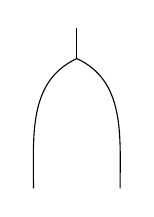
\begin{tikzpicture}[scale=.55]
		\draw (1,3.7) to (1,3);
		\draw (1,3) to [out=205, in=90] (0,0);
		\draw (1,3) to [out=-25, in=90] (2,0);
	\end{tikzpicture}
	\hspace*{1cm}
	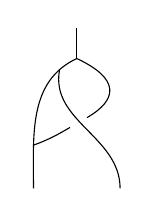
\begin{tikzpicture}[scale=.55]
		\draw (1,3.7) to (1,3);
		\draw (1,3) to [out=205, in=90] (0,0);
		\draw [shorten >= 0cm] (.6,2.73) to [out=-100, in=90] (2,0);
		\draw [shorten >= .15cm] (1,3) to [out=-25, in=30, distance=1.1cm] (1,1.5);
		\draw [shorten <= .1cm] (1,1.5) to [out=210, in=20] (0,1);
	\end{tikzpicture}
	\hspace*{1cm}
	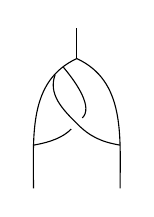
\begin{tikzpicture}[scale=.55]
		\draw (1,3.7) to (1,3);
		\draw (1,3) to [out=205, in=90] (0,0);
		\draw (1,3) to [out=-25, in=90] (2,0);
		\draw [shorten >= 0cm] (.5,2.63) to [out=-110, in=135] (1,1.5);
		\draw [shorten <= 0cm] (1,1.5) to [out=-45, in=170] (2,1);
		\draw [shorten >= .1cm] (.69,2.8) to [out=-50, in=45] (1,1.5);
		\draw [shorten <= .1cm] (1,1.5) to [out=-135, in=10] (0,1);
	\end{tikzpicture}
	\hspace*{1cm}
	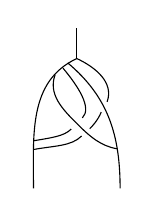
\begin{tikzpicture}[scale=.55]
		\draw (1,3.7) to (1,3);
		\draw (1,3) to [out=205, in=90] (0,0);
		\draw [shorten >= 0cm] (.5,2.63) to [out=-110, in=135] (1,1.5);
		\draw [shorten >= .05cm] (1,1.5) to [out=-45, in=170] (2.02,.9);
		\draw [shorten >= .1cm] (.68,2.78) to [out=-50, in=45] (1,1.5);
		\draw [shorten <= .1cm] (1,1.5) to [out=-135, in=10] (0,1.1);
		\draw (.79,2.9) to [out=-40, in=90] (2,0);
		\draw (1,3) to [out=-25, in=70] (1.7,2);
		\draw [shorten <= .15cm] (1.7,2) to [out=-120, in=45] (1.3,1.38);
		\draw [shorten <= .1cm] (1.24,1.34) to [out=-135, in=10] (0,.9);
	\end{tikzpicture}
}
\end{document}
	\caption{Graphs representing cup-$i$ coproducts.}
	\label{f:cup-i}
\end{figure}

It is not known if the cup-$i$ coproducts defined in \cref{e:closed cup-i} agree with those previously constructed, for which a comparison is also missing.
This highlights the value of a potential axiomatic characterization of cubical cup-$i$ coproducts as it exists in the simplicial case \cite{medina2022axiomatic}.

As already mentioned, cup-$i$ coproducts represent the Steenrod squares at the chain level,
which are primary operations in mod~2 cohomology.
To obtain secondary cohomology operations one studies the cohomological relations these operations satisfy, for example the Cartan and Adem relations \cite{steenrod1962cohomology}.
To do this at the cubical cochain level, as it was done in \cite{medina2020cartan,medina2021adem} for the simplicial case, the operadic viewpoint is important, so our $E_\infty$-structure on cubical cochains invites the construction of cochain representatives for secondary operations in the cubical case.

For $p$ an odd prime, Steenrod also introduced operations on the mod~$p$ cohomology of spaces using the homology of symmetric groups \cite{steenrod1952reduced, steenrod1953cyclic}.
Using the operadic framework of May \cite{may1970general}, we described in \cite{medina2021may_st} elements in $\UM$ representing multicooperations defining Steenrod operations at any prime.
In particular, as proven in this work, these so-called \textit{cup-$(p,i)$ coproducts} are defined on cubical chains and are expressible, similarly to \cref{e:closed cup-i}, in terms of $\Delta$, the permutations of factors, and $\ast$.
The aforementioned construction of cubical cup-$(p,i)$ coproducts has been implemented in the open source computer algebra system \href{https://comch.readthedocs.io/en/latest/}{\texttt{ComCH}} \cite{medina2021comch}.
